\section{基本OSPF协议} % (fold)
\label{sec:ospf}
	\subsection{协议概述} % (fold)
	\label{sub:协议概述}
		本项目中实现的OSPF协议是一个基于链路状态的路由协议,运行该协议的每个路由器能够根据收到的所有链路信息计算出一个最短路径树,构造对应的转发表。其链路的权重的赋值取决于带宽,算法使用的是Dijkstra算法和RPF广播算法,定义了Hello和LS(link-state)两种报文格式。实现了多条等费用路径的路由选择,并且解决了路由循环问题和改善了路由震荡问题。在协议的扩展中,实现了该协议下适用的traceRoute功能。
	% subsection 协议概述 (end)
	\subsection{算法} % (fold)
	\label{sub:算法}
		\subsubsection{路由计算算法} % (fold)
		\label{ssub:路由计算算法}
			在原生LS算法中,一个路由器的路由计算的方法是:以自身为起点,执行Dijkstra算法以得到一棵最短路径树,然后根据最短路径树得到转发表。采用这种方法,计算出的到每个目的地的最短路径是唯一的。
			\par 为了实现多条等费用最短路径选择,本项目采用以下算法过程:
			\begin{itemize}
				\item 对于路由器的每个邻居$nb$,以$nb$为起点执行Dijkstra算法,得到$nb$到其他路由器的最短路径距离$dist_{nb}$。
				\item 使用Bellman-Ford更新公式,计算自身到其他路由器的距离:$$dist_{self}(dest) = \min_{nb}\{dist_{nb}(dest) + metric(self,nb)\} $$
				\item 对于每一个目的地$dest$,依次判断每个邻居是否能作为下一跳(即该邻居是否在一条最短路径上)。判断一个邻居$nb$能作为下一跳的依据是:$nb$能到达$dest$并且满足公式$$dist_{self}(dest) = dist_{nb}(dest) + metric(self,nb)$$将符合条件的邻居加入转发表中去往$dest$的下一跳列表。
			\end{itemize}		
		% subsubsection 路由计算算法 (end)
		\subsubsection{广播算法} % (fold)
		\label{ssub:广播算法}
			使用了RPF(Reverse Path First)算法,收到一个广播数据包的路由器会向来路以外的路由器转发该广播数据包当且仅当来路位于广播源和当前路有器的任一条最短路径上。
		% subsubsection 广播算法 (end)
	% subsection 算法 (end)
	\subsection{协议特性} % (fold)
	\label{sub:协议特性}
		\subsubsection{协议流程} % (fold)
		\label{ssub:协议流程}
		本项目中实现的OSPF协议主要包含的流程如下:
		\begin{enumerate}
			\item 路由器在进入区域时,向所有邻居发送hello报文(该报文用于向邻居声明自己的存在),再向该区域内的路由器广播自己的链路信息。
			\item 该路由器会定时地发送hello报文和广播链路信息。
			\item 收到一个hello报文意味着要维持该邻居的状态;而如果在一段时间内没有收到某个邻居路由器的hello报文,则认为该路由器故障或离开该区域。
			\item 当自身的链路信息发生改变时,广播链路信息;当收到其它路由器的链路信息时,根据该信息更新自己的关于该区域的链路信息数据库。
		\end{enumerate}		
		% subsubsection 协议流程 (end)
	% subsection 协议特性 (end)
	\subsection{报文格式} % (fold)
	\label{sub:报文格式}
		该协议中包含的Hello报文、LS报文、traceRoute报文、Echo报文、普通数据报文格式如下:
		\par Hello 报文。
	\begin{table}[H]
	\centering
		\begin{tabular}{|c|}
			\hline
			Command \\
			\hline
			Source address \\
			\hline
			Metric \\
			\hline
		\end{tabular}		
	\end{table}

	LSU报文(广播报文)。
	\begin{table}[H]
	\centering
	\begin{tabular}{|c|}
		\hline                 
		Command                \\
		\hline                 
		Source address         \\
		\hline                 
		Transmit address       \\
		\hline                 
		Destination address    \\
		\hline                 
		Metric                 \\
		\hline                 
		Repeat of last 8 bytes \\
		\hline                 
		$\cdots$               \\
		\hline                 
	\end{tabular}		
\end{table}

TraceRoute报文
\begin{table}[H]
	\centering
	\begin{tabular}{|c|}
		\hline              
		Command             \\
		\hline              
		source address      \\
		\hline              
		destination address \\
		\hline              
		count               \\
		\hline              
	\end{tabular}		
\end{table}	

Echo 报文
\begin{table}[H]
	\centering
	\begin{tabular}{|c|}
		\hline              
		Command             \\
		\hline              
		source address      \\
		\hline              
		destination address \\
		\hline              
		local address       \\
		\hline              
	\end{tabular}		
\end{table}
普通报文的格式与在RIP中的格式相同。
报文项解释:
\begin{enumerate}[(1)]
	\item Command(1 Byte):指明这条报文的类型。
	      \begin{enumerate}[]
	      	\item 0: 普通报文
	      	\item 1: hello
	      	\item 2: LSU(Link State Update)
	      	\item 3: traceRoute
	      	\item 4: Echo
	      \end{enumerate}
	\item Source address(6 Bytes):指明发送方的源地址和监听端口。
	\item Destination address(6 Bytes):指明目的地的源地址和监听端口。
	\item Transmit address(6 Bytes):指明广播中转发者的源地址和监听端口。
	\item Local address(6 Bytes):指明Echo报文发送者的源地址和监听端口。
	\item Metric(2 Bytes):代价度量。
	\item Count(1 Bytes):路由跳数。
	\end{enumerate}
	
	% subsection 报文格式 (end)
	\subsection{协议扩展} % (fold)
	\label{sub:协议扩展}
		\begin{enumerate}
			\item 路由循环
			\item 路由震荡\\
				·为了避免路由震荡,设置路由器广播其链路信息的时间随机化。
			\item TraceRoute\\
				·由于OSPF没有跳数这一说法,向目的地发跳数为1-32共32个报文,当一个路由器收到该报文,则提取其中的跳数,并将它减一。\\
				·如果跳数为0,则向报文的源地址返回一个Echo报文;如果跳数>0且报文的目的地址不等于当前路由的地址,将跳数打包进原报文中,
				继续向目的地转发;否则,判定为多余的traceRoute报文,将之舍弃。\\
				·源地址路由器收集所有返回的Echo报文,如果5s内收到目的地址返回的Echo报文,则输出该路径;否则认为该目的地址不可达。
		\end{enumerate}
	% subsection 协议扩展 (end)
	\subsection{协议实现} % (fold)
	\label{sub:协议实现}
		本OSPF协议基本由Python实现,主要利用的是socket进行套接字编程、struct库进行数据的打包和解包、threading库管理线程和定时器。
		\par 实现方法实现了一个OSPF协议类,处理内部流程和为外部调用留出了收发数据、查询路由等接口。
	% subsection 协议实现 (end)
	\subsection{结果} % (fold)
	\label{sub:结果}
		测试所用的拓扑图以及路由结果如下图\ref{fig:ospfTest1}和\ref{fig:ospfTest2}所示。
		\begin{figure}[H]
			\centering
			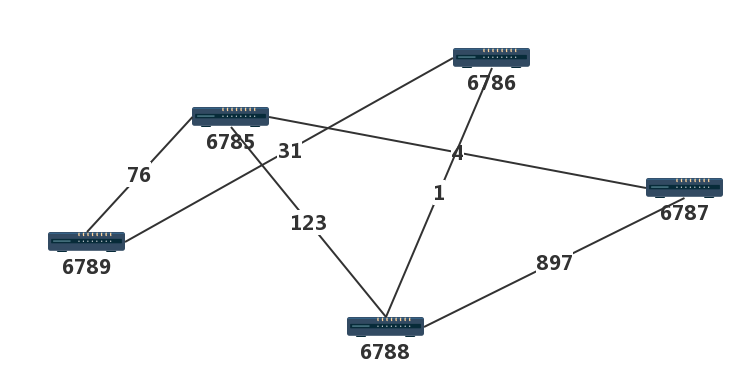
\includegraphics[scale=0.4]{imgs/topo2/tpop1.png}
			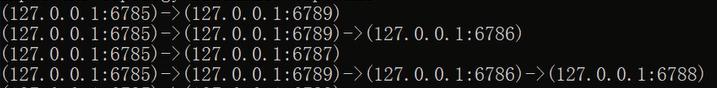
\includegraphics[scale=1]{imgs/ospfTest1.PNG}
			\caption{OSPF测试样例一}
			\label{fig:ospfTest1}
		\end{figure}
		\begin{figure}[H]
			\centering
			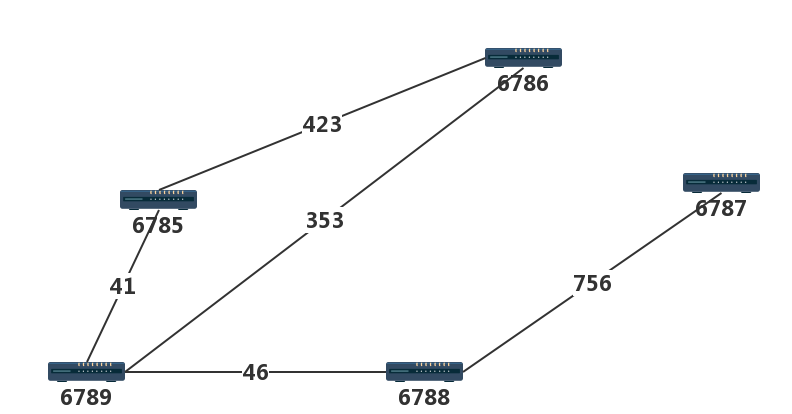
\includegraphics[scale=0.4]{imgs/topo2/topo2.png}
			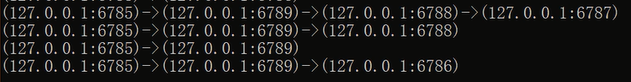
\includegraphics[scale=1]{imgs/ospfTest2.PNG}
			\caption{OSPF测试样例二}
			\label{fig:ospfTest2}
		\end{figure}
		成功找出了其中的最短路径。
	% subsection 结果 (end)
	\subsection{总结} % (fold)
	\label{sub:总结}
		% TODO 和真正OSPF协议的区别
		\begin{itemize}
			\item 本项目中实现的基本OSPF协议淡化了其区域概念,简化了报文类型和路由器类型,同时也简化了路由器状态。
			\item 原生的LS算法会导致路由震荡和路由循环问题,而我们实现的OSPF协议改善甚至基本解决了这类问题。
		\end{itemize}
		
% subsection 总结 (end)
	

% section ospf (end)
